\pagestyle{fancy}
\headheight 20pt
\lhead{Ph.D. Thesis --- R. Woods }
\rhead{McMaster - Physics \& Astronomy}
\chead{}
\lfoot{}
\cfoot{\thepage}
\rfoot{}
\renewcommand{\headrulewidth}{0.1pt}
\renewcommand{\footrulewidth}{0.1pt}

\chapter{Applications to Galaxy Formation and Future Projects}
\label{chap:galaxyformation}
\thispagestyle{fancy}

We now use the algorithm described in chapter \ref{chap:method} and tested in chapter \ref{chap:codetests} to carry out simulations of an isolated galaxy. We have chosen to start with an isolated galaxy in order to probe the FUV field present in a [Milky Way-like... z=1?] disk in order to check if it is an important SF regulation mechanism.

FUV is an interesting band to start with for a few reasons. While FUV does not ionize gas, it is the primary driver of photoelectric heating \citep{tielens05}, which is the dominant heating mechanism for the ISM and the warm neutral medium. Despite this, very few astrophysical simulations actually include photoelectric heating due to its dependence on a radiation field.

As well, FUV is typically able to penetrate further into the ISM. At common densities in the ISM, an optical depth of 1 is typically only achieved after roughly one kpc. Current simulations, especially of isolated galaxies, can resolve distances much smaller than this, so looking at effects due to FUV is very feasible. On the other hand, bands such as EUV are usually absorbed within a few pc, a resolution that is very costly for even isolated galaxy simulations.

In order to create a realistic ISM, a two-phase instability must be present so that both the Cold Neutral Medium (CNM) at roughly  and the Warm Neutral Medium (WNM) can be present at pressure equilibrium.

We have chosen to use an isolated galaxy IC from the AGORA galaxy comparison project \citep{kimEt14} to ensure use of a well-tested IC and provide a larger base for comparison of results.

\section{FUV Fields in the AGORA Disk}
\label{sec:agora}

The AGORA galaxy comparison project is a large computational comparison project that aims ``to raise the realism and predictive power of galaxy simulations and the understanding of the feedback processes that regulate galaxy `metabolism,' and by doing so to solve long-standing problems in galaxy formation'' \citep{kimEt14}. To accomplish this, the project has created both isolated and cosmological galaxy formation initial conditions at many different masses and resolutions, and has attempted to standardize physics modules and analysis methods for all of the codes involved in the project.

\subsection{Initial Conditions and Physics}
\label{sec:initialconditions}

We have chosen to run the isolated disk initial condition in order to examine FUV's effect on the ISM. The specific details of the ICs for this disk can be found in \citet{kimEt14}, section 2.2. We summarize here the important information.

The initial conditions have been generated at three different resolutions using the \textsc{MakeDisk} code, written by Volker Springel. The disk is created with four components: a dark matter halo, a gas disk, a stellar disk, and stellar bulge. The low resolution disk has $10^5$ DM particles, $10^5$ stellar disk particles, $10^5$ gas particles, and $1.24\e{4}$ stellar bulge particles. The medium and high resolution disks have 10 and 100 times more particles in each component, respectively.

The DM follows a NFW profile \citep{navarroEt97} with a concentration parameter $c = 10$ and a spin parameter $\lambda = 0.04$. The disk has an exponential profile with a scale length of $r_d = 3.432$ kpc and a scale height of $z_d = 0.1 r_d$. The disk is split into the stellar component, which has a mass of $4.297\e{10} M_{\odot}$, and a gas component, which has a mass of 20\% of the DM mass. The stellar bulge follows the Hernquist \citeyear{hernquist90} density profile with a bulge-to-disk mass ratio of B/D = 0.1. Gas is initiated at $10^4$ K. The \textsc{MakeDisk} code ensures that the above conditions give quasi-equilibrium [what does that mean?] for the four components. 

We have run the IC for 335~Myr in order to make sure it was relaxed, and started all subsequent runs from this point. An image of the relaxed IC is shown in figure \ref{fig:agoraic}.

\begin{figure}
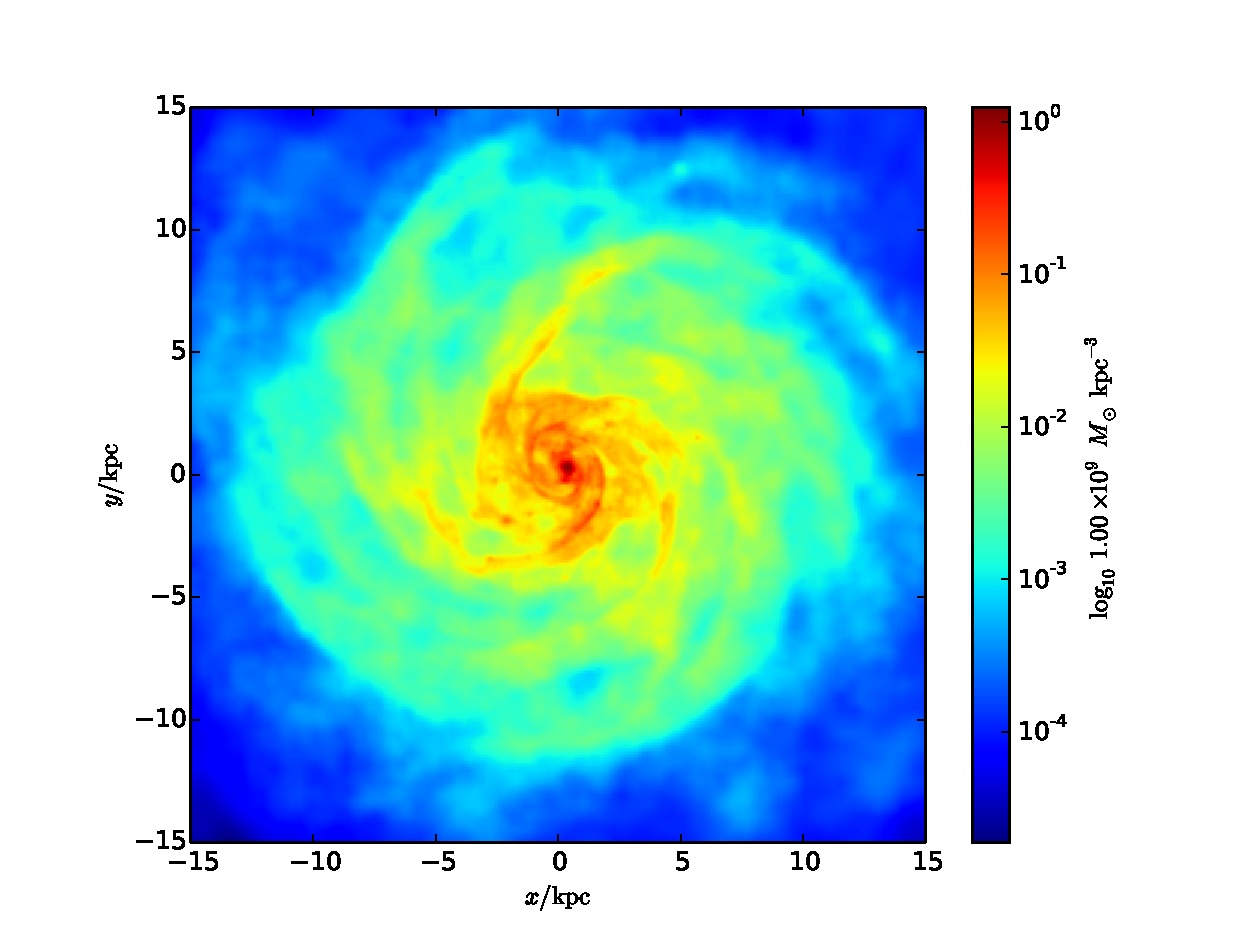
\includegraphics[width=\textwidth]{graphics/AGORAic.eps}
\caption[The AGORA IC]{A density projection of a relaxed version of the AGORA initial condition. We have run the IC for 335 Myr in order to relax it.}
\label{fig:agoraic}
\end{figure}

%notes about various runs we did

We have run the low resolution simulation with a number of different physical parameters, including our radiative transfer with FUV, a prescribed FUV field, Supernovae (SNe) feedback using superbubbles \citep{kellerEt14}, and a number of different opacities. Table \ref{tab:simsummary} summarizes the simulations and the names we have given them.

\begin{table}
\begin{tabular}{llllp{3cm}}
Name & RT & Opacity (g/cm$^{2}$) & SNe Feedback & Notes\\ \hline \hline
FUV0 & No & 0 & No &\\
FUVop400 & Yes & 400 & No & Wolfire Opacity\\
FUVop300 & Yes & 300 & No & \\
8FUVop300 & Yes & 300 & No & 8 x resolution\\
FUVop100 & Yes & 100 & No & \\
FUVthin & Yes & 0 & No & \\
8FUVthin & Yes & 300 & No & 8 x resolution\\
FUV2e-26 & No & 300 & No & Prescribed FUV\\
FB & No & 300 & yes & \\
FB\_FUVop300 & Yes & 300 & yes & \\
\hline
\end{tabular}
\caption[Summary of simulations]{A summary of the simulations that were run. RT is ``Radiative Transfer'', FUV Strength denotes the strength of the }
\label{tab:simsummary}
\end{table}

FUV0 is the base run, with no feedback of any sort included. FUV2e-26 is previously used way of including a UV field, where the UV field from \citet{wolfireEt03} is imposed on the galaxy as a function of radius. All FUVopxxx runs use our radiative transfer algorithm, and the opxxx represents the value that opacity has been set to in g~cm$^{-2}$. The FUVthin runs represent runs where we have turned the opacity of the intervening gas off, so that there is no absorption of photons (apart from at the receiving particles). Runs prefixed with an 8 are higher resolution versions, with eight times as many gas particles. The FB runs include superbubble SNe feedback with an energy per supernova of $0.5\e{51}$ ergs, half of the typical value associated with SNe.

In runs that used our radiative transfer, a luminosity function for FUV was adopted based on Starburst99 \citep{leithererEt99}. A function was fit to the FUV luminosity of a star cluster vs time, per unit solar mass. Figure \ref{fig:bandenergies} includes the cumulative version of the FUV luminosity that was used (the pink line).

We attempted to match opacities given in \citet{wolfireEt03}. The left pane of figure \ref{fig:wolfiresummary} shows the midplane HI density and absorption coefficient, and the right pane is the inferred opacity from the left pane, obtained by dividing absorption by mass density.

\begin{figure}
        \centering
        \begin{subfigure}[b]{0.45\textwidth}
                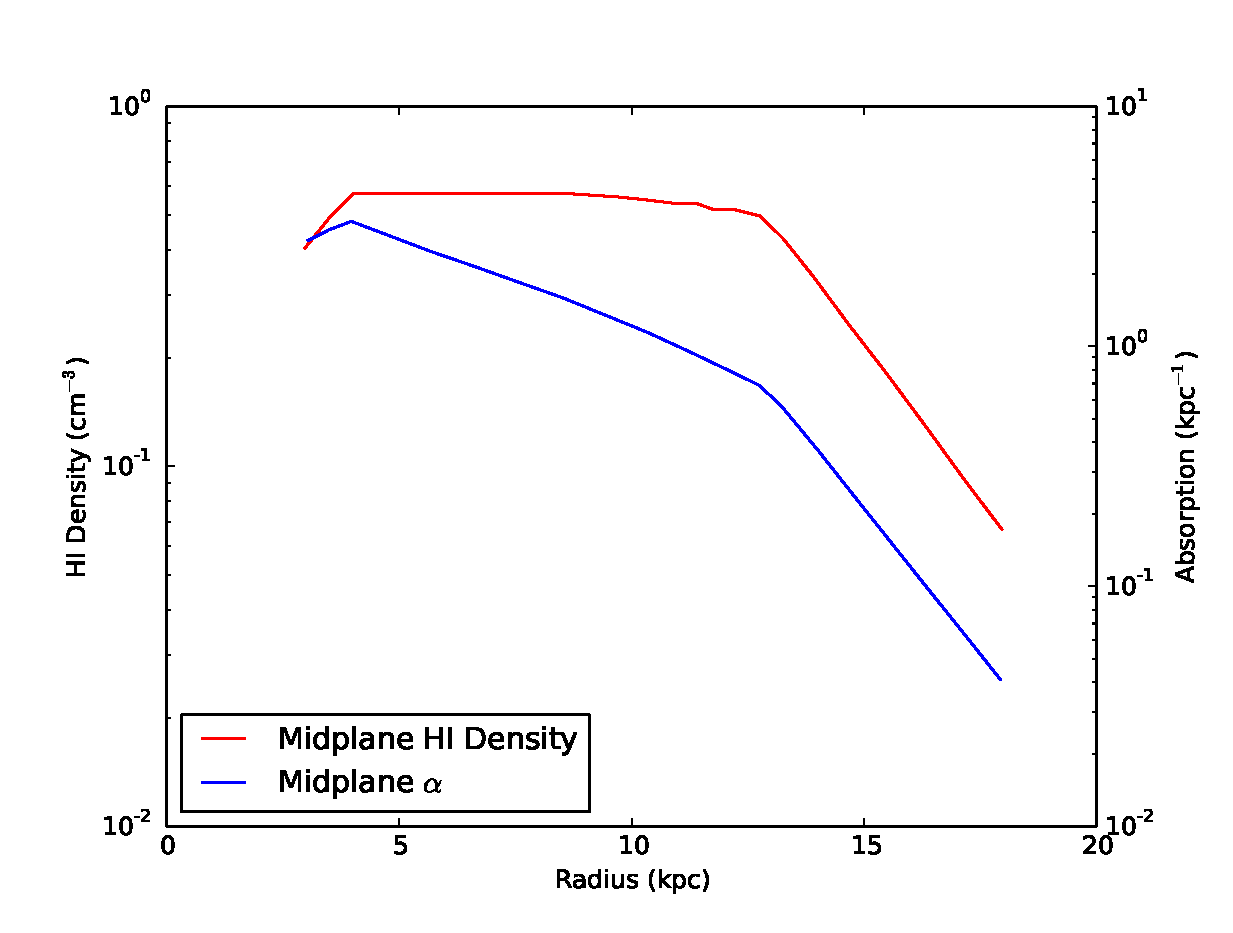
\includegraphics[width=\textwidth]{graphics/densityabsorptionvr.eps}
        \end{subfigure}
        ~ 
        \begin{subfigure}[b]{0.45\textwidth}
                \includegraphics[width=\textwidth]{graphics/opacityvr.eps}
        \end{subfigure}
        \caption[Parameters from \citet{wolfireEt03}.]{Parameters from \citet{wolfireEt03}. The left plot shows the mid plane number density and absorption coefficient. The right plot is obtained by converting number density to a mass density and dividing absorption coefficient by mass density.}
        \label{fig:wolfiresummary}
\end{figure}

Note that the profile in opacity is due solely to a scaling in metallicity of the local opacity. \citet{wolfireEt03} assume that opacity changes as

\begin{equation}
\kappa = \kappa_{\odot}\left(\frac{Z}{Z_{\odot}}\right),
\end{equation}

\noindent
where $\kappa_{\odot}$ is the metallicity in the solar neighborhood, inferred to be ~400 g/cm$^{-2}$ from figure \ref{fig:wolfiresummary}. The value of 400 g/cm$^{-2}$ includes contributions from both absorption and scattering, where each make up roughly 50\% of the total [cite here - draine?]. Since we have aimed only to model absorption, we are only concerned with photons removed from the medium. In a disk, scattering can do this by scattering photons up, out of the disk. Thus, the effective opacity for our simulation should be somewhere between the full opacity and the opacity with absorption only, which would be roughly 200 g/cm$^{-2}$. We have adopted 300 g/cm$^{-2}$ as our standard value for runs.

We have also included runs at eight times higher resolution to check on convergence of results. These runs are prefixed with an ``8''.

\section{The Role of FUV on Star Formation}
\label{sec:fuvsfr}

We begin by looking at the star formation history of each simulation. Figure \ref{fig:sfrvtime} shows the star formation rate as a function of time for each simulation. 

\begin{figure}
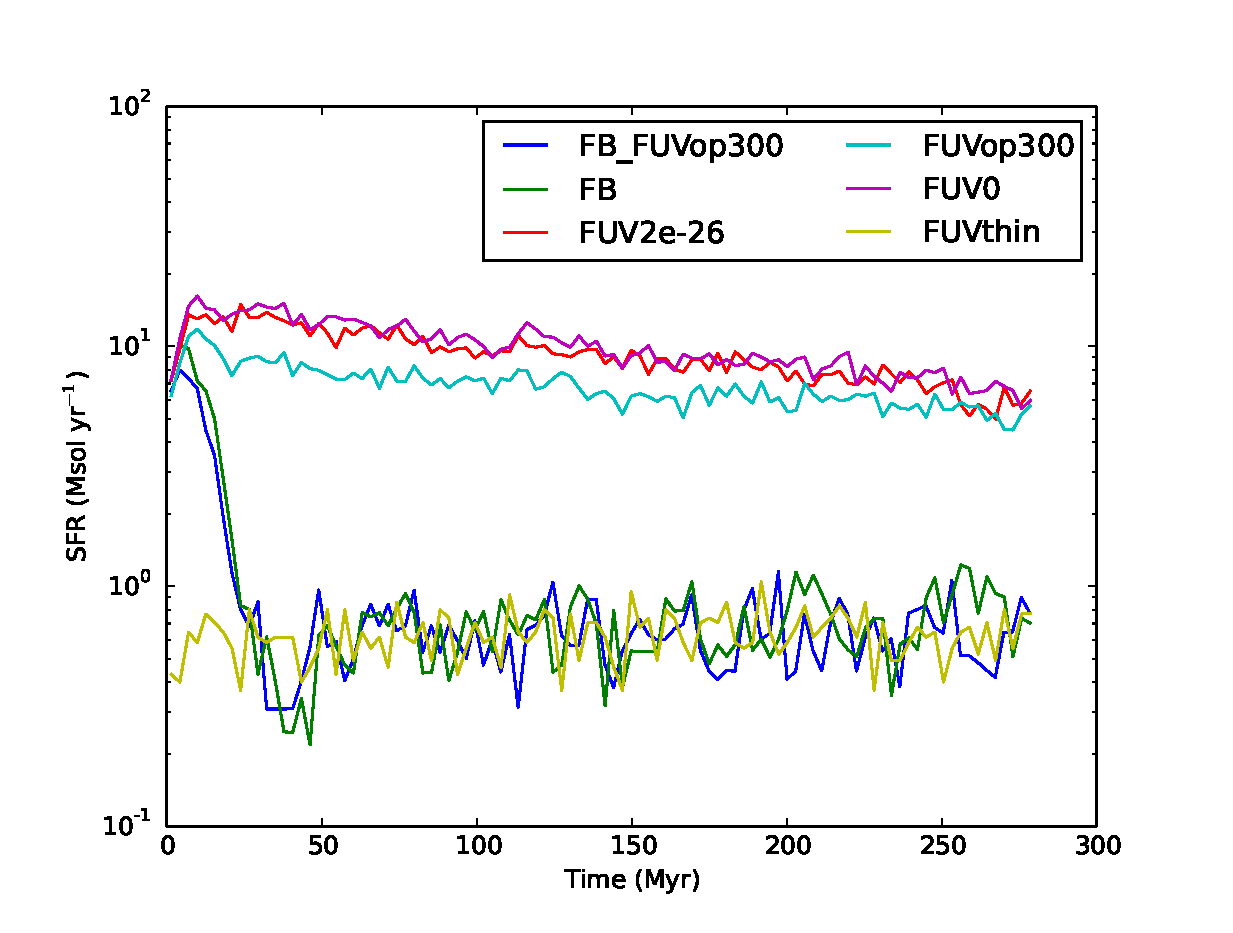
\includegraphics[width=\textwidth]{graphics/sfrvtime.eps}
\caption[Star formation histories.]{Star formation rate vs time for each simulation.}
\label{fig:sfrvtime}
\end{figure}

Without any sort of regulation mechanism, the galaxy forms stars at about 10 $M_{\odot}~yr^{-1}$. The milky way is thought to be forming stars at roughly $1.9 \pm 0.4~M_{\odot}~yr^{-1}$ \citep{chomiukPovich11}, so the unregulated value in the AGORA disk is much higher than one would expect for a realistic disk. 

The introduction of a prescribed UV field (FUV2e-26) has little to no effect on star formation. However, calculating the FUV field via our radiative transfer scheme does have a noticeable effect, depending on opacity. Using an opacity of 300 cm$^2$ g$^{-1}$ (FUVop300), we see a reduction in the SFR of roughly 10-25\%. To bracket possibilities, we next consider the optically thin case (FUVthin). In this case, star formation is hugely regulated, dropping from 10 $M_{\odot}~yr^{-1}$ to 0.5 $M_{\odot}~yr^{-1}$, or a factor of 20. The same is true for all runs containing SNe feedback.

While it's clear that SNe are excellent at regulating star formation, figure \ref{fig:sfrvtime} begs the question of whether or not SNe feedback is \emph{necessary} at its current strength. One of the discussion points in recent literature has been around how SNe can drive outflows and regulate star formation. However, in most cases, obtaining a reasonable SFR with SNe as the regulation mechanism has been done at the expense of driving far too much gas out of the galaxy \citep{scannapiecoEt12}, or by requiring unphysically high amounts of energy per SN coupled with early EUV \citep{stinsonEt13}. 

\begin{figure}
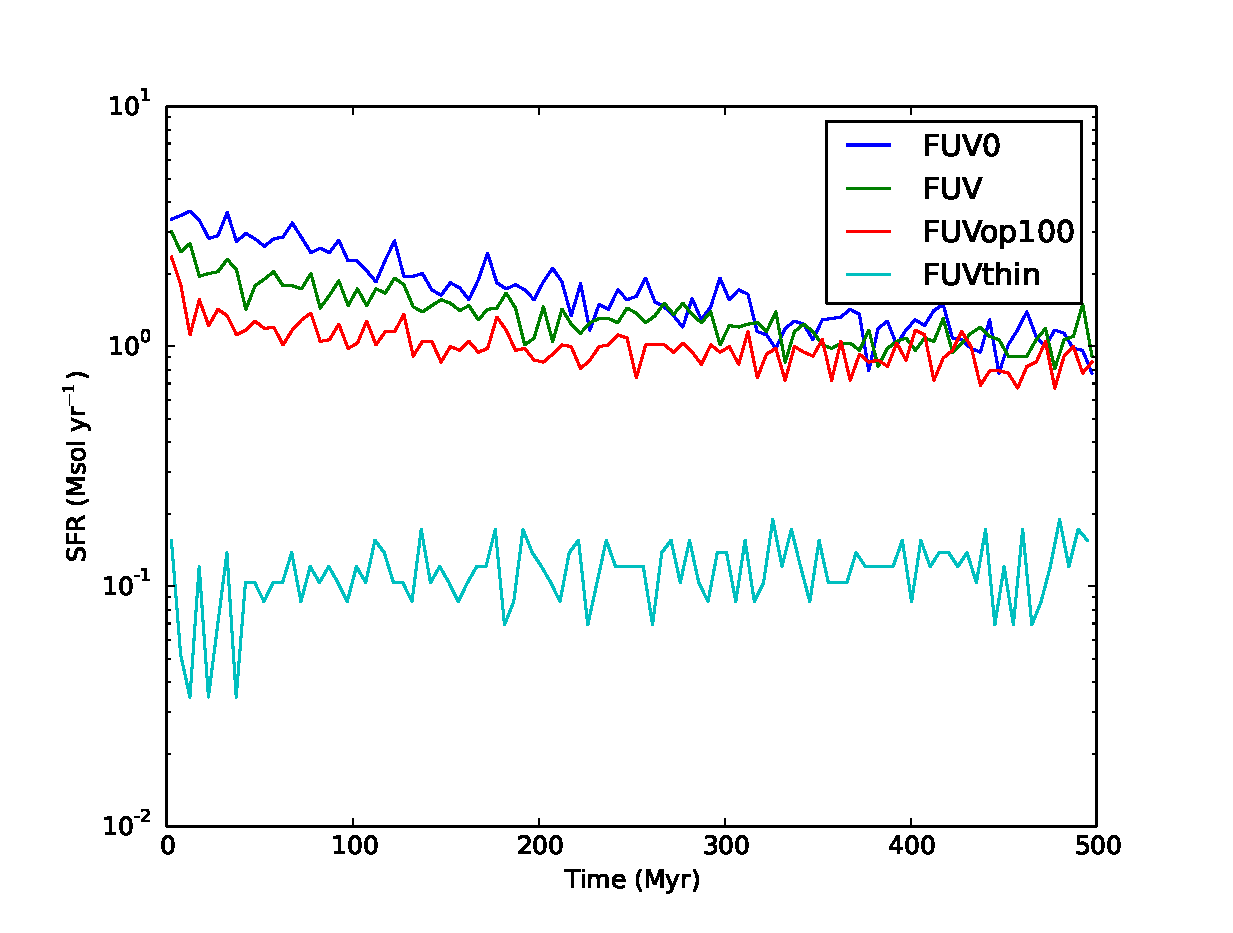
\includegraphics[width=\textwidth]{graphics/sfrvtimeRT.eps}
\caption[Star formation histories.]{Star formation rate vs time for each simulation.}
\label{fig:sfrvtimeRT}
\end{figure}

Figure \ref{fig:sfrvtimeRT} shows the star formation history as a function of differing opacities (and code resolutions). As with figure \ref{fig:sfrvtime}, we include the base run (FUV0) and an optically thin run to show the extremes. Figure \ref{fig:sfrvtimeRT} shows an almost linear relationship between opacity and SFH. Depending on the value of opacity, FUV can be anywhere between a modest, 10-15\% effect, up to a 95\% effect.

However, just because something is regulating star formation doesn't mean it is physical. Figure \ref{fig:intensityvopacity} is a plot of FUV intensity vs radius in the midplane of the galaxy for the four different opacities.

\begin{figure}
        \centering
        \begin{subfigure}[b]{0.45\textwidth}
                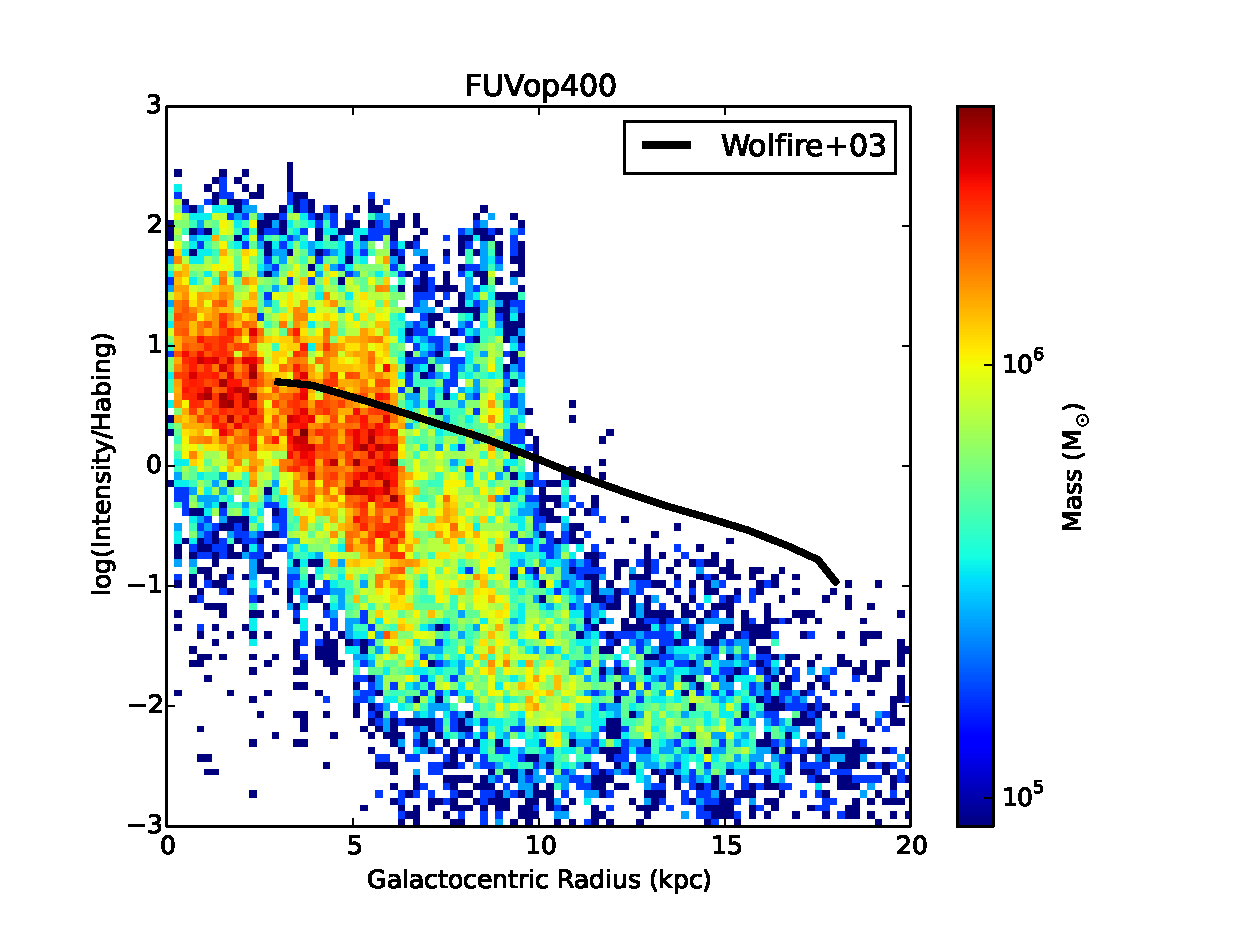
\includegraphics[width=\textwidth]{graphics/intensityvrRadFUVop400_J300200.eps}
                \caption{FUVop400}
                \label{fig:intensityop400}
        \end{subfigure}
        ~ 
        \begin{subfigure}[b]{0.45\textwidth}
                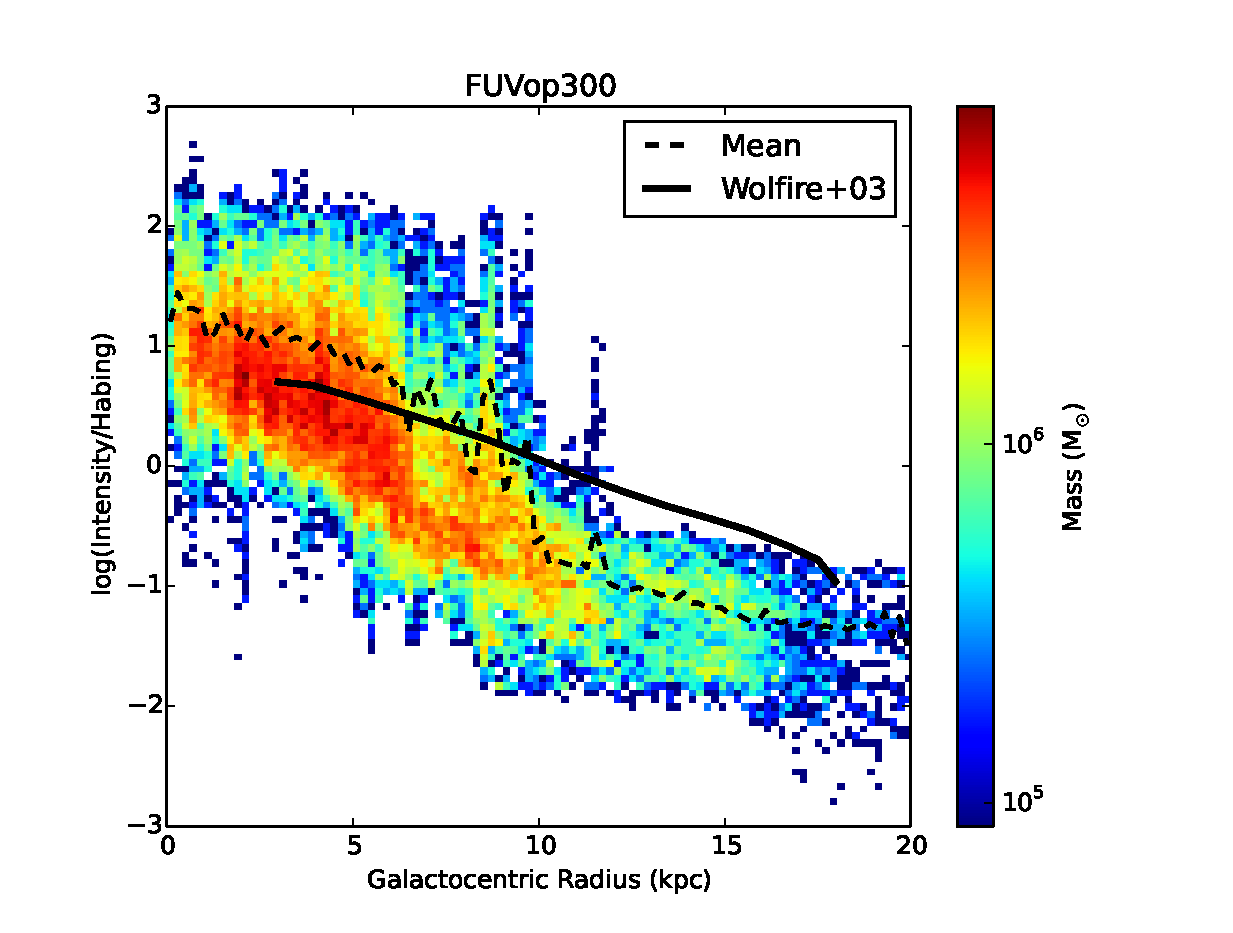
\includegraphics[width=\textwidth]{graphics/intensityvrRadFUV_J300200.eps}
                \caption{FUVop300}
                \label{fig:intensityop300}
        \end{subfigure}
        \\
        \begin{subfigure}[b]{0.45\textwidth}
                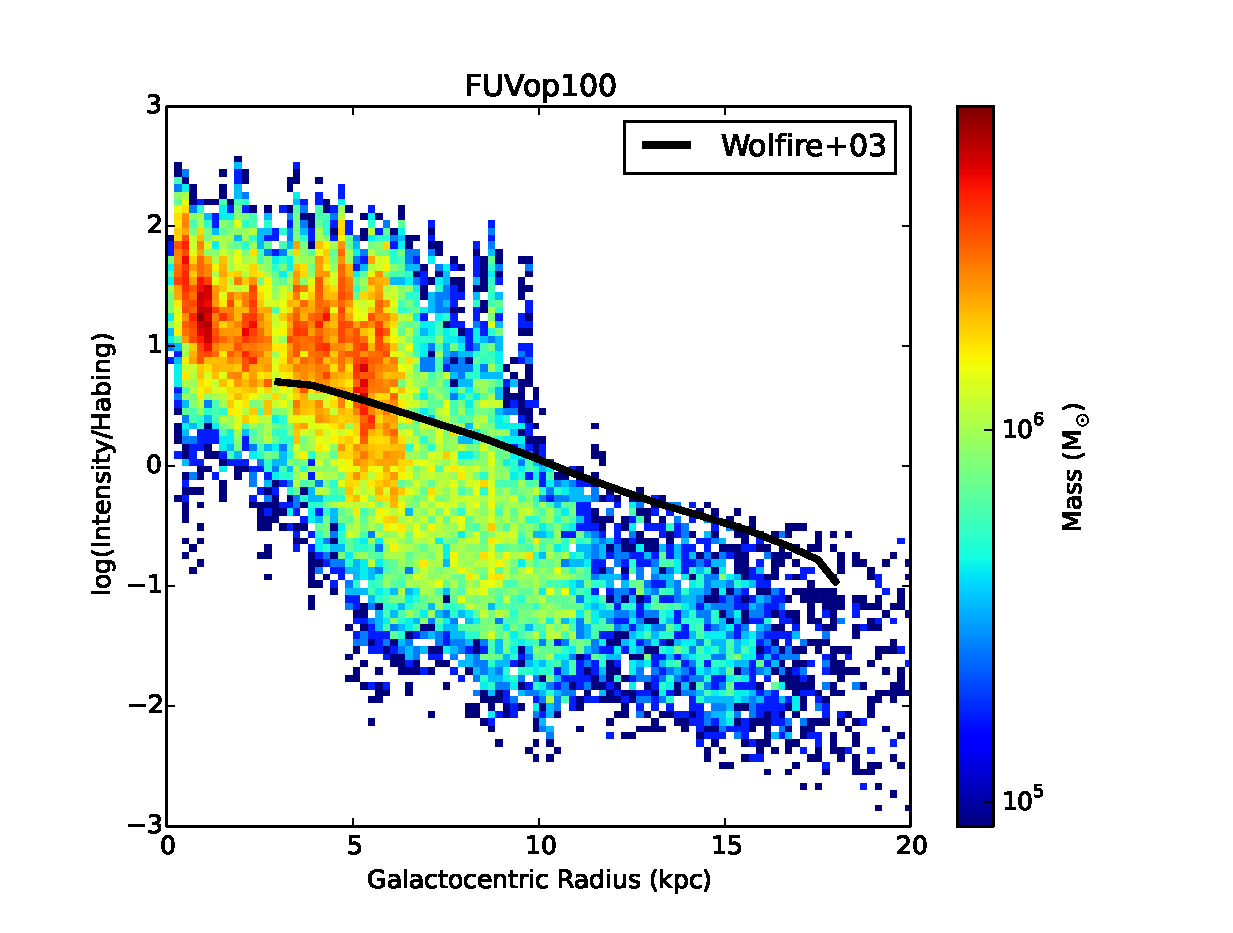
\includegraphics[width=\textwidth]{graphics/intensityvrRadFUVop100_J300200.eps}
                \caption{FUVop100}
                \label{fig:intensityop100}
        \end{subfigure}
        ~
        \begin{subfigure}[b]{0.45\textwidth}
                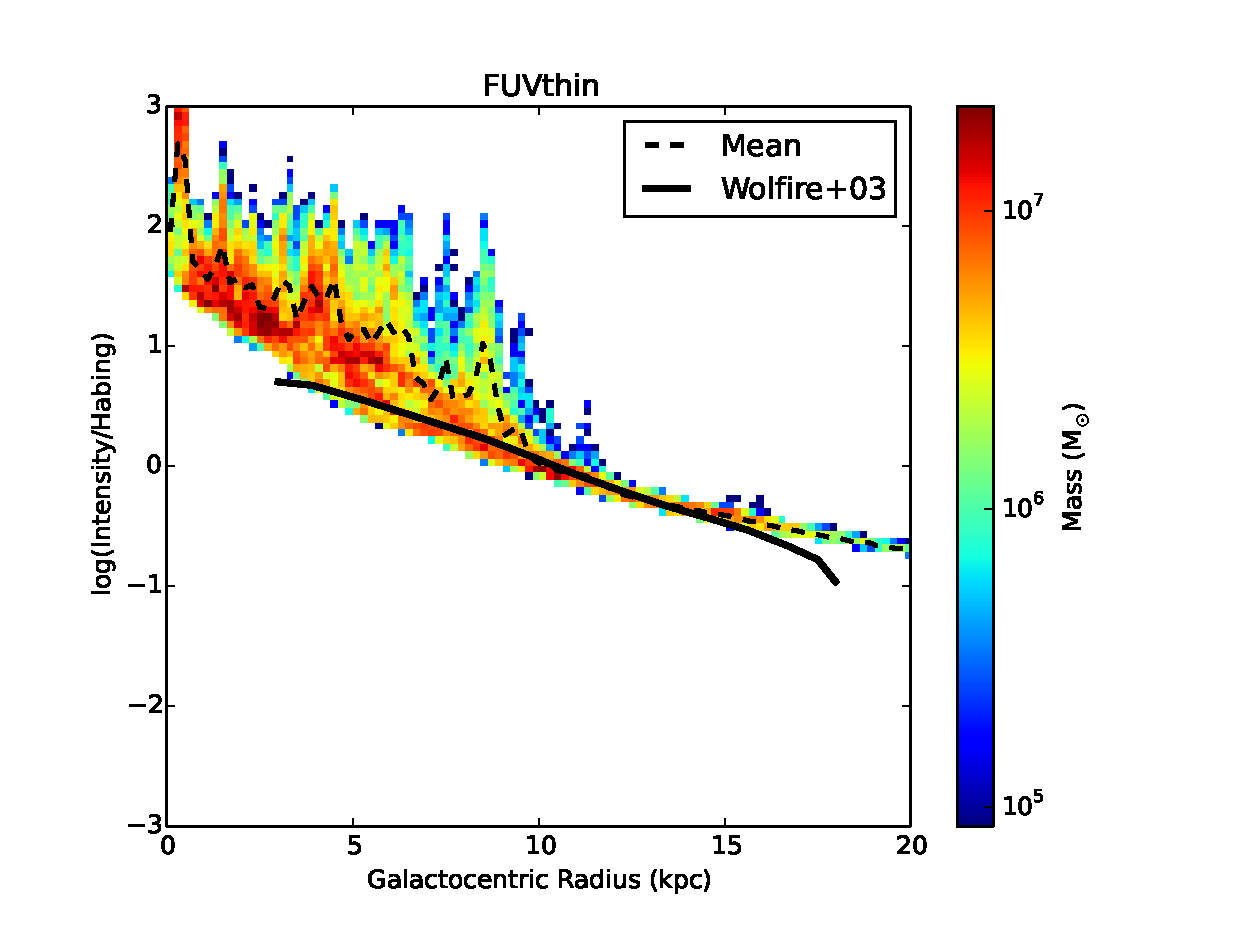
\includegraphics[width=\textwidth]{graphics/intensityvrRadFUVthin_J300200.eps}
                \caption{FUVthin}
                \label{fig:intensitythin}
        \end{subfigure}
        \caption[Intensity with varying opacity.]{A 2-D histogram of FUV intensity vs radius in the galaxy midplane for $\kappa = 100 - 400$ g/cm$^{-2}$ and for an optically thin medium. The color represents the amount of mass in each bin, and the line is average midplane field from \citet{wolfireEt03}.}
        \label{fig:intensityvopacity}
\end{figure}

The particles have been binned into 2-D intensity-radius bins and the line is the mean intensity presented in \citet{wolfireEt03}. Note that we have divided our measured intensity by the Habing Field value measured at the solar radius, $4\pi 1.2\e{-4} erg~s^{-1}~cm^{-2}$. If the opacities from the simulations are realistic, they should also produce realistic FUV profiles.

We see that star formation is intense enough in the inner part of the galaxy ($r < 10$ kpc) that opacity does not actually have a drastic effect. Intensity stays largely consistent independent of opacity. However, the outer region ($r>10$ kpc) of the galaxy sees a large change with opacity; the average intensity jumps by a factor of almost 10 for a factor of four change in opacity (comparing the op100 case to the op 400 case).

It's also quite interesting to note the large intensity drop between 5 and 10 kpc in all but the optically thin case. This feature is not present in the profile presented by \citet{wolfireEt03}. [Add more here].

\begin{figure}
        \centering
        \begin{subfigure}[b]{0.45\textwidth}
                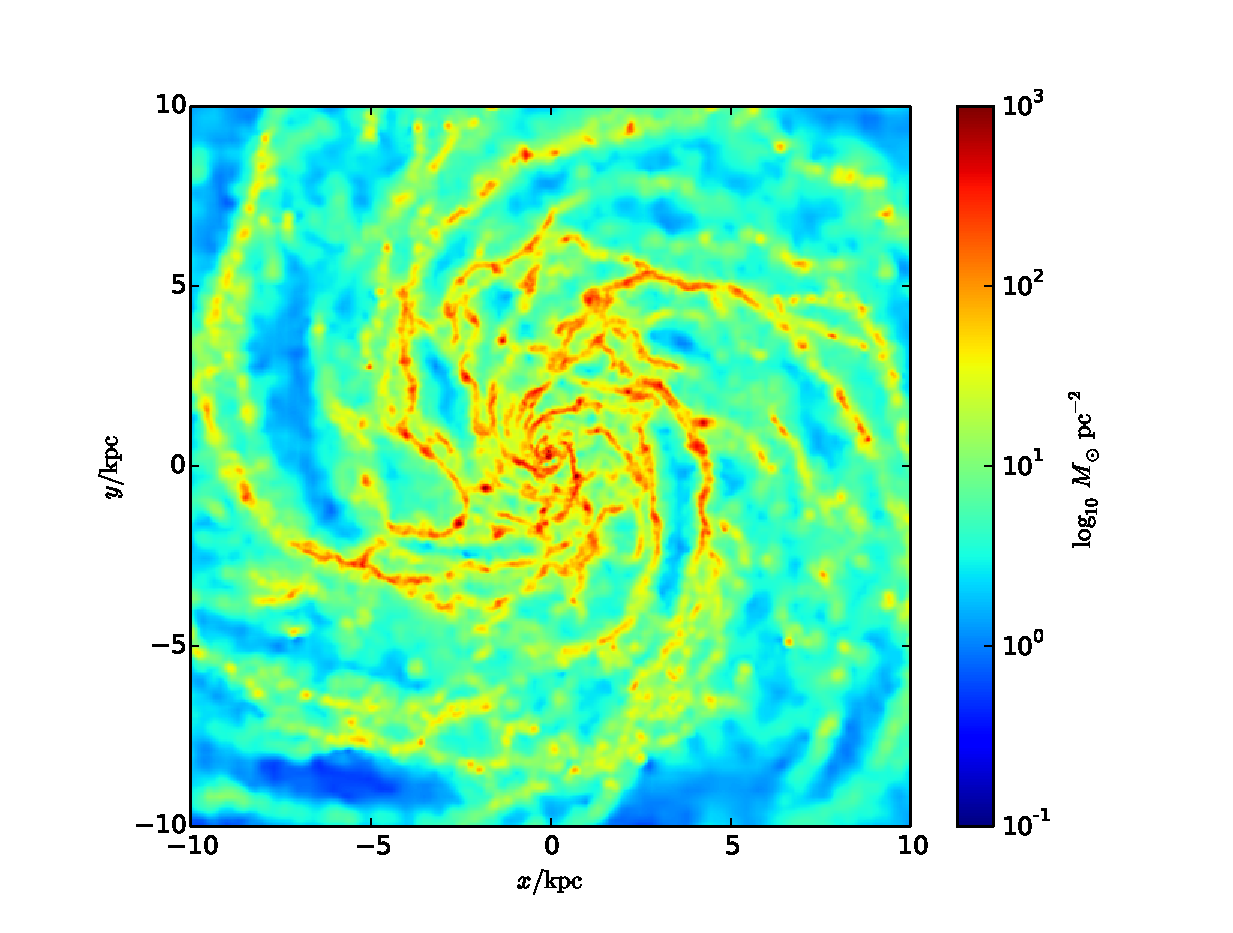
\includegraphics[width=\textwidth]{graphics/surfacedensityRadFUV_J300200.eps}
                \caption{Gas Surface Density}
                \label{fig:op300surface}
        \end{subfigure}
        ~ 
        \begin{subfigure}[b]{0.45\textwidth}
                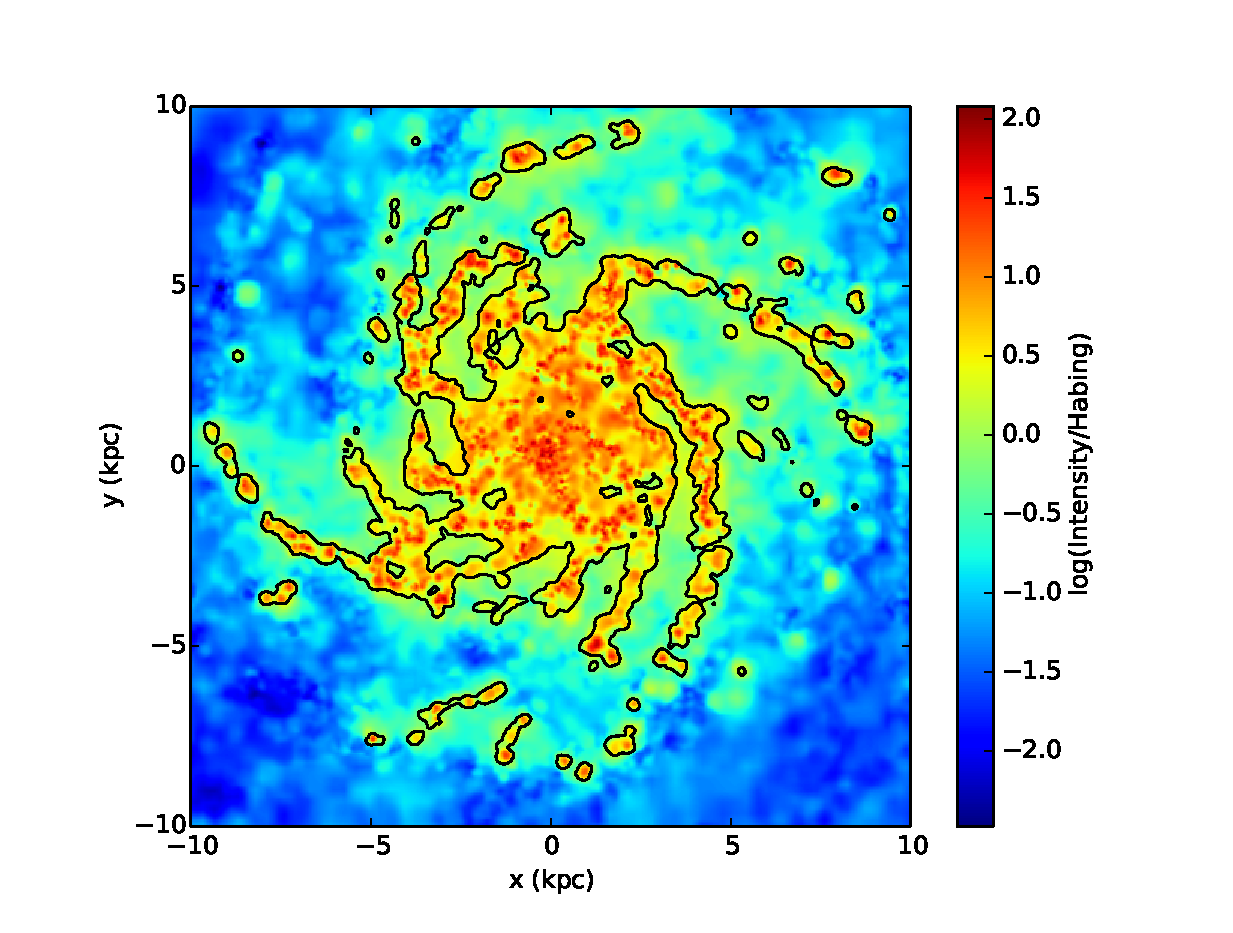
\includegraphics[width=\textwidth]{graphics/intensityRadFUV_J300200.eps}
                \caption{Intensity}
                \label{fig:op300intensity}
        \end{subfigure}
        \\
        \begin{subfigure}[b]{0.45\textwidth}
                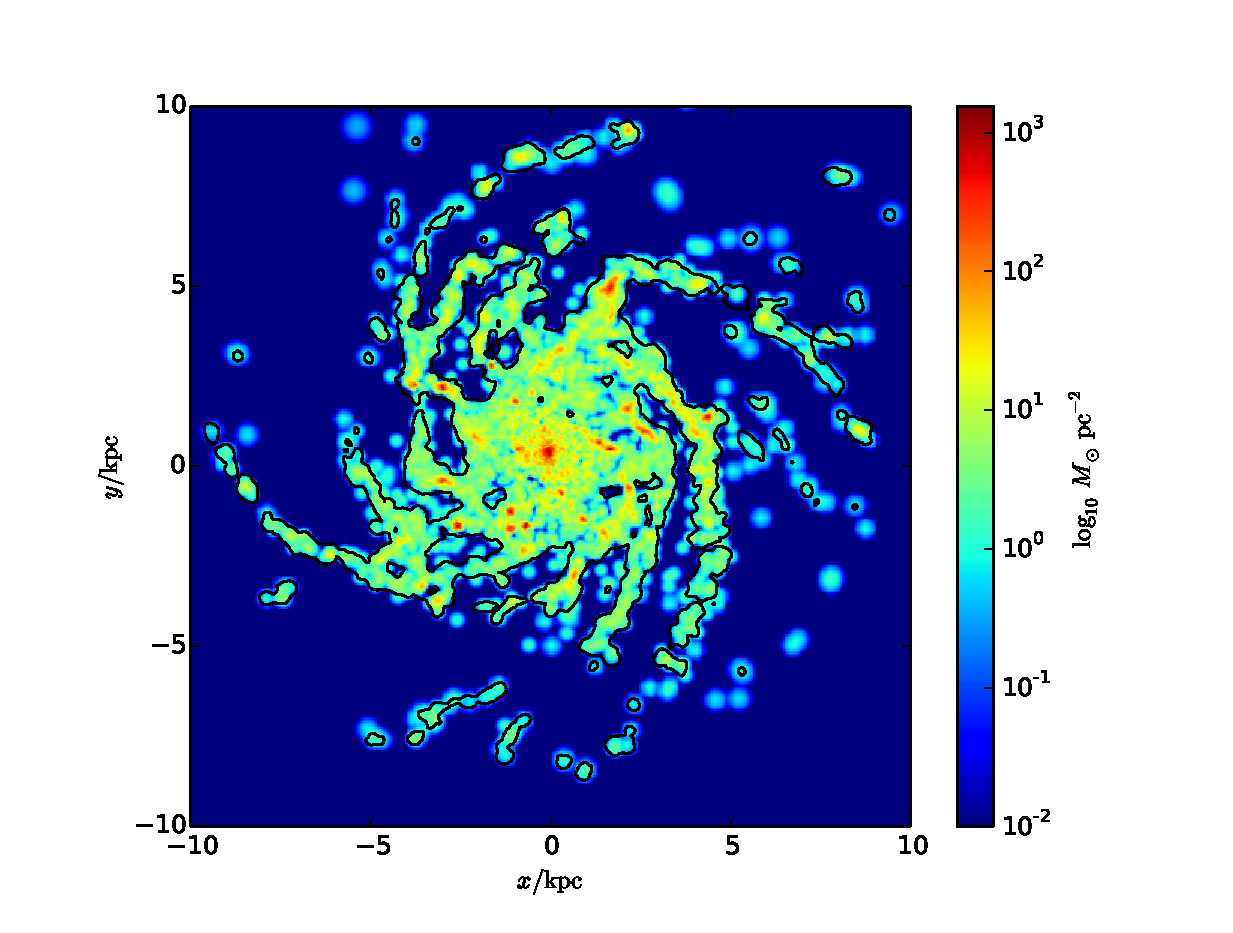
\includegraphics[width=\textwidth]{graphics/stellardensityRadFUV_J300200.eps}
                \caption{Stellar Surface Density}
                \label{fig:op300stellar}
        \end{subfigure}
        ~
        \begin{subfigure}[b]{0.45\textwidth}
                \includegraphics[width=\textwidth]{graphics/stellarsigmaRadFUV_J300200.eps}
                \caption{Surface Density Profiles}
                \label{fig:op300sigma}
        \end{subfigure}
        \caption[FUVop300 Images and profiles]{The above are...}
        \label{fig:op300detail}
\end{figure}

Figure \ref{fig:op300detail} shows face on images of different properties of the FUVop300 case at t = 200 Myr. Figure \ref{fig:op300surface} is a gas surface density plot, \ref{fig:op300intensity} is log intensity, with a contour of gas surface density drawn at 20 $M_{\odot}~pc^{-2}$, \ref{fig:op300stellar} is stellar surface density with the same contour, and \ref{fig:op300sigma} are radial profiles of the gas and stellar surface density.

In order to understand the specific effect FUV has on gas, we consider phase diagrams for gas in the galaxy. Figure \ref{fig:phasediagrams} shows phase diagrams of gas in a number of the different simulations.

\begin{figure}
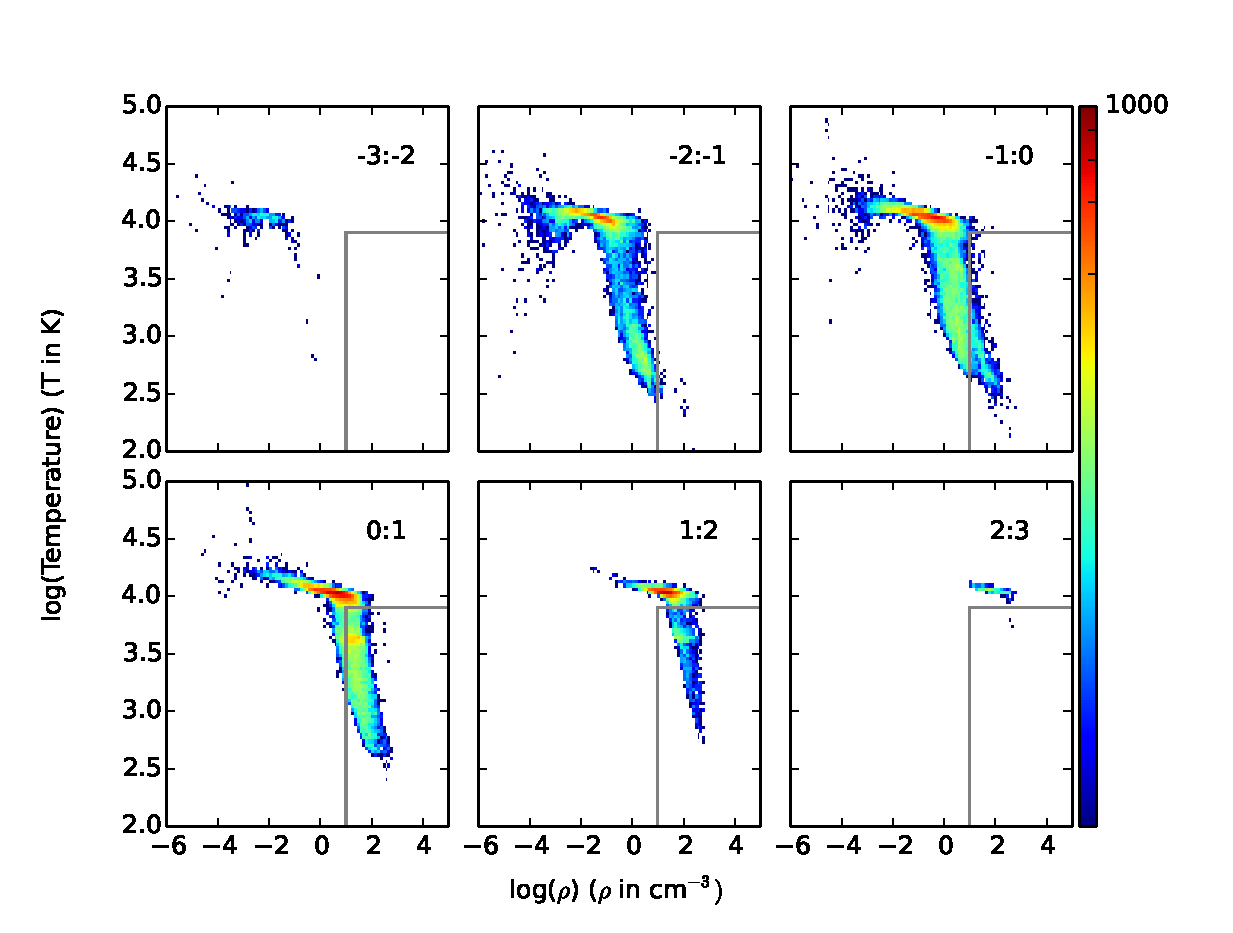
\includegraphics[width=\textwidth]{graphics/phaseRadFUV_J300200.eps}
\caption[Phase diagrams of gas with different FUV intensity.]{Phase diagrams for FUVop300 at varying FUV intensities. Each panel shows the gas state for a different magnitude of FUV intensity.}
\label{fig:phasediagrams}
\end{figure}

We see that high FUV intensity is present in the highest density gas (which can be confirmed in figure \ref{fig:op300intensity}). This is not surprising, as high FUV intensity is due to young stars, which form in dense gas. [Not sure if this plot says much else....]

\section{Discussion}
\label{sec:discussion}


[Add commentary. Re-radiation important? Clumpy medium vs average opacity not the same.]


%\begin{figure}
%        \centering
%        \begin{subfigure}[b]{0.3\textwidth}
%                \includegraphics[width=\textwidth]{graphics/surfacedensityRadFUV0_J300080.eps}
%                \caption{FUV0}
%                \label{fig:intensitythin}
%        \end{subfigure}
%        ~
%        \begin{subfigure}[b]{0.3\textwidth}
%                \includegraphics[width=\textwidth]{graphics/surfacedensityRadFUV2e-26_J300080.eps}
%                \caption{FUV2e-26}
%                \label{fig:intensity100}
%        \end{subfigure} 
%        ~ 
%        \begin{subfigure}[b]{0.3\textwidth}
%                \includegraphics[width=\textwidth]{graphics/surfacedensityRadFUVop400_J300080.eps}
%                \caption{FUVop400}
%                \label{fig:intensity100}
%        \end{subfigure}
%        \\
%        \begin{subfigure}[b]{0.3\textwidth}
%                \includegraphics[width=\textwidth]{graphics/surfacedensityRadFUV_J300080.eps}
%                \caption{FUVop300}
%                \label{fig:intensitythin}
%        \end{subfigure}
%        ~
%        \begin{subfigure}[b]{0.3\textwidth}
%                \includegraphics[width=\textwidth]{graphics/surfacedensityRadFUVop100_J300080.eps}
%                \caption{FUVop100}
%                \label{fig:intensitythin}
%        \end{subfigure}
%        ~
%        \begin{subfigure}[b]{0.3\textwidth}
%                \includegraphics[width=\textwidth]{graphics/surfacedensityRadFUVthin_J300080.eps}
%                \caption{FUVthin}
%                \label{fig:intensitythin}
%        \end{subfigure}Y
%        \\
%         \begin{subfigure}[b]{0.3\textwidth}
%                \includegraphics[width=\textwidth]{graphics/surfacedensityRadFB_J300080.eps}
%                \caption{FB}
%                \label{fig:intensity100}
%        \end{subfigure}
%        ~ 
%        \begin{subfigure}[b]{0.3\textwidth}
%                \includegraphics[width=\textwidth]{graphics/surfacedensityRadFB_FUV2e-26_J300080.eps}
%                \caption{FB\_FUV2e-26}
%                \label{fig:intensitythin}
%        \end{subfigure}
%        ~
%        \begin{subfigure}[b]{0.3\textwidth}
%                \includegraphics[width=\textwidth]{graphics/surfacedensityRadFB_FUV_J300080.eps}
%                \caption{FB\_FUV}
%                \label{fig:intensitythin}
%        \end{subfigure}
%        \caption[Surface density for varying runs.]{Surface density plots for the different runs.}
%        \label{fig:intensityvopacity}
%\end{figure}

%\begin{figure}
%        \centering
%        \begin{subfigure}[b]{0.45\textwidth}
%                \includegraphics[width=\textwidth]{graphics/fluximageRadFUV_J300080.eps}
%                \caption{FUVop300}
%                \label{fig:intensitythin}
%        \end{subfigure}
%        ~
%        \begin{subfigure}[b]{0.45\textwidth}
%                \includegraphics[width=\textwidth]{graphics/fluximageRadFUVthin_J300080.eps}
%                \caption{FUVthin}
%                \label{fig:intensity100}
%        \end{subfigure}        
%        \\
%        \begin{subfigure}[b]{0.45\textwidth}
%                \includegraphics[width=\textwidth]{graphics/fluximage8_RadFUV_J300080.eps}
%                \caption{8\_FUVop300}
%                \label{fig:intensitythin}
%        \end{subfigure}
%        ~
%        \begin{subfigure}[b]{0.45\textwidth}
%                \includegraphics[width=\textwidth]{graphics/fluximage8_RadFUVthin_J300080.eps}
%                \caption{8\_FUVthin}
%                \label{fig:intensitythin}
%        \end{subfigure}        
%        \\ 
%        \begin{subfigure}[b]{0.45\textwidth}
%                \includegraphics[width=\textwidth]{graphics/fluximageRadFUVop400_J300080.eps}
%                \caption{FUVop400}
%                \label{fig:intensity100}
%        \end{subfigure}
%        ~
%        \begin{subfigure}[b]{0.45\textwidth}
%                \includegraphics[width=\textwidth]{graphics/fluximageRadFB_FUV_J300080.eps}
%                \caption{FB\_FUVop300}
%                \label{fig:intensitythin}
%        \end{subfigure}    
%        \caption[Mass-weighted intensity.]{Mass-weighted intensity of the different runs.}
%        \label{fig:intensityvopacity}
%\end{figure}